
\documentclass[a4paper,UKenglish]{lipics-v2018}
%This is a template for producing LIPIcs articles. 
%See lipics-manual.pdf for further information.
%for A4 paper format use option "a4paper", for US-letter use option "letterpaper"
%for british hyphenation rules use option "UKenglish", for american hyphenation rules use option "USenglish",
% for section-numbered lemmas etc., use "numberwithinsect"

\usepackage{microtype,amssymb,amsmath,stmaryrd,mathpartir,array,graphicx}%if unwanted, comment out or use option "draft"
\usepackage[table]{xcolor}
\newcommand{\xt}[1]{\texttt{#1}}
\newcommand{\tupleo}[1]{\xt{Tuple1\{}#1\xt{\}}}
\newcommand{\tuplet}[2]{\xt{Tuple2\{}#1,#2\xt{\}}}
\newcommand{\union}[2]{\xt{Union\{}#1,#2\xt{\}}}
\newcommand{\denotes}[1]{\llbracket #1 \rrbracket}

\newcommand{\bsub}{<:_b}
\newcommand{\nsub}{<:_n}

\newcommand{\goodcell}{\cellcolor{green!25}}
\newcommand{\badcell}{\cellcolor{red!25}}

%\graphicspath{{./graphics/}}%helpful if your graphic files are in another directory

\bibliographystyle{plainurl}% the recommnded bibstyle

\title{Subtyping Correctness - Temporary Title}

\titlerunning{Temporary Title}%optional, please use if title is longer than one line

\author{Benjamin Chung}{Northeastern University}{bchung@ccs.neu.edu}{}{}%mandatory, please use full name; only 1 author per \author macro; first two parameters are mandatory, other parameters can be empty.

\author{Francesco Zappa Nardelli}{Inria}{}{}{}

\author{Jan Vitek}{Northeastern University \& Czech Technical University}{}{}{}

\authorrunning{B. Chung, F. Zappa Nardelli, J. Vitek}%mandatory. First: Use abbreviated first/middle names. Second (only i,n severe cases): Use first author plus 'et al.'

\Copyright{Benjamin Chung, Francesco Zappa Nardelli, Jan Vitek}%mandatory, please use full first names. LIPIcs license is "CC-BY";  http://creativecommons.org/licenses/by/3.0/

\subjclass{Dummy classification}% mandatory: Please choose ACM 2012 classifications from https://www.acm.org/publications/class-2012 or https://dl.acm.org/ccs/ccs_flat.cfm . E.g., cite as "General and reference $\rightarrow$ General literature" or \ccsdesc[100]{General and reference~General literature}. 

\keywords{Dummy keyword}%mandatory

\category{}%optional, e.g. invited paper

\relatedversion{}%optional, e.g. full version hosted on arXiv, HAL, or other respository/website

\supplement{}%optional, e.g. related research data, source code, ... hosted on a repository like zenodo, figshare, GitHub, ...

\funding{}%optional, to capture a funding statement, which applies to all authors. Please enter author specific funding statements as fifth argument of the \author macro.

% put the algorithm up front and explanation
% here's a cute and simple algorithm that works for distributive tuples and unions
% write it with imperative stacks
% tuple union is hard known for 20yrs sol w/ normalization
% prob 1: state explosion (also seen in swift) CDeuce approach doesn't work
% prob 2: expressivity interacting with rhicher type system normalization doesn't work at all
% what we show is an alternative way to deal with distributive subtyping
% sol prob 1: lazy stack-based subtyping algorithm
% sol prob 2: ....
%
\acknowledgements{}%optional

%Editor-only macros:: begin (do not touch as author)%%%%%%%%%%%%%%%%%%%%%%%%%%%%%%%%%%
\EventEditors{John Q. Open and Joan R. Access}
\EventNoEds{2}
\EventLongTitle{42nd Conference on Very Important Topics (CVIT 2016)}
\EventShortTitle{CVIT 2016}
\EventAcronym{CVIT}
\EventYear{2016}
\EventDate{December 24--27, 2016}
\EventLocation{Little Whinging, United Kingdom}
\EventLogo{}
\SeriesVolume{42}
\ArticleNo{23}
%\nolinenumbers %uncomment to disable line numbering
%\hideLIPIcs  %uncomment to remove references to LIPIcs series (logo, DOI, ...), e.g. when preparing a pre-final version to be uploaded to arXiv or another public repository
%%%%%%%%%%%%%%%%%%%%%%%%%%%%%%%%%%%%%%%%%%%%%%%%%%%%%%

\begin{document}

\maketitle
\begin{abstract}
We describe a novel algorithm for deciding subtyping for a type language consisting
of tuples, unions, and existential type variables without normalization and requiring
space linear in the size of the input types. We prove algorithmic correctness with 
respect to a semantic notion of subtyping using a proof assistant. Finally, we examine
the algorithm's use in the Julia programming language.
\end{abstract}

\section{FZN Introduction}
%%% Please do not edit from here...

Subtyping union types has been known for a long time.  Recall the rules.

If we add covariant tuples, again, distributivity has been known for a
long time.  Show the problem with standard rules.

The standard solution is to rewrite types in normal form.  Explain
normal form.

This has two inconvenients:
\begin{itemize}
\item Space explosion.

  \item Lack of completeness in presence of more expressive types,
    eg.\ existential (explain Julia counterexample).
\end{itemize}

While subtyping union types is inherently exponential in time, it does
not have to suffer from the above limitation wrt.\ space and
expressiveness.

In this paper we describe how the algorithm used by the Julia language to
decide subtype solves subtyping union types and tuples.  We prove in
Coq that the alogrithm is correct and complete with respect to a standard
semantics subtyping model.  

%%% ...to here
%%% END FZN Introduction    

\section{Prior Work}

Previous efforts to provide a decision procedure for distributive unions rely
heavily on normalization. In order to decide subtyping in one of these
approaches, the type is first normalized (to integrate the distributivity
axiom) and then the standard syntax-directed subtyping algorithm is applied to
conclude the subtyping
relation~\cite{muehlboeck2018empowering,Reynolds1997,Pierce1991}. This
normalization step puts the type into disjunctive normal form thereby allowing
the algorithmic union rule to decide subtyping correctly. As there are
exponentially many choice sets for any given type (where one of two choices
may be given at each union), the space taken up by the fully normalized type
can be substantial. Moreover, (in languages with some kind of higher-rank
polymorphism) the normalization process eliminates all internal unions; as a
concequence, variable instantiations may be over-specialized and some
semantically-valid subtyping relations may not hold.



\section{Algorithm}

Our algorithm for deciding subtyping works by iterating through every possible
choice that could be made between branches of unions within a type and
incrementally checking that the requisite guarantees hold at each type. In
this section, we will describe the implementation of the algorithm in OCaml.
In the following section, we will then discuss the Coq version of the same
algorithm.

The type language for our algorithm is a subset of that used in the Julia
programming language. We focus on the distributive property of unions over
tuples. Notably, our type system does not include arrow types---Julia has none
---nor type variables. Additionally, so as to avoid needing an additional
externally-provided subtype hierarchy, we specify that atomic types (atoms)
are subtypes only if they are identical.

\hspace{1em}

\begin{minipage}{\textwidth}
\begin{minipage}{0.4\textwidth}
\begin{verbatim}
type typ =
  | Atom of int
  | Tuple1 of typ
  | Tuple2 of typ * typ
  | Union of typ * typ

type st_choice = Left | Right
\end{verbatim}
\end{minipage}
\begin{minipage}{0.5\textwidth}
\begin{verbatim}
let rec initial_choice (a:typ) =
  match a with
  | Atom i -> []
  | Tuple1 t -> initial_choice t
  | Tuple2(t1,t2) -> (initial_choice t1) 
  		@ (initial_choice t2)
  | Union(l,r) -> Left::(initial_choice l)
\end{verbatim}
\end{minipage}
\end{minipage}
\hspace{1em}

\noindent The key construct for our algorithm is the \verb|st_choice|
operation, which represents whether the algorithm takes the left or the right
branch of a union. The algorithm stores the choice made at each union at the
present iteration in two stacks of \verb|st_choice|s, one for each side of the
subtype relation. 

\begin{verbatim}
let rec last_left_to_right (acc:st_choice list) (ll : st_choice list option) = function
  | Left::tl -> last_left_to_right (Left::acc) (Some (Right::acc)) tl
  | Right::tl -> last_left_to_right (Right::acc) ll tl
  | [] -> option_map List.rev ll
let rec extend_list (a:typ) (ls:st_choice list) = match (a,ls) with
  | (Atom i, _) -> ([], ls)
  | (Tuple1 t, _) -> extend_list t ls
  | (Tuple2(t1,t2), _) -> let (hd,tl) = extend_list t1 ls in
                          let (hd2,tl2) = extend_list t2 tl in
                          (hd @ hd2, tl2)
  | (Union(l,r), Left::rs) -> let (hd,tl) = extend_list l rs in (Left::hd,tl)
  | (Union(l,r), Right::rs) -> let (hd,tl) = extend_list r rs in (Right::hd,tl)
  | (Union(l,r), []) -> (Left::initial_choice l,[])

let rec next_state (a:typ) (ls:st_choice list) =
  option_map fst (option_map (extend_list a) (last_left_to_right [] None ls))
\end{verbatim}

To move through all possible choices, the \verb|next_state| function steps a
stack of \verb|st_choice|s to the next state. Here, we arbitrarily define next
state as ``the deepest unexplored alternative,'' or, equivalently, where the
last left has been converted to a right. We implement \verb|next_state| in two
distinct helper functions, the first of which implements the last-left-to-
right operation and the second implements a fix-up operation.

\begin{figure}
\begin{tabular}{cccc}
& \hspace{5em} & &\\
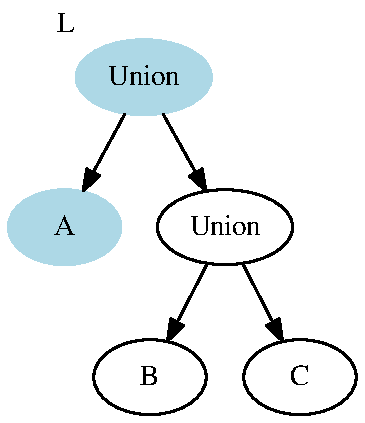
\includegraphics[scale=0.6]{figures-gen/example1.pdf} &
\multicolumn{2}{c}{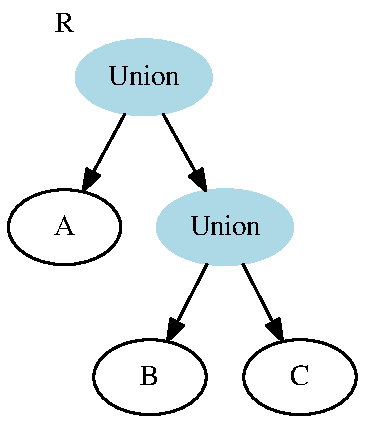
\includegraphics[scale=0.6]{figures-gen/example2.pdf}} &
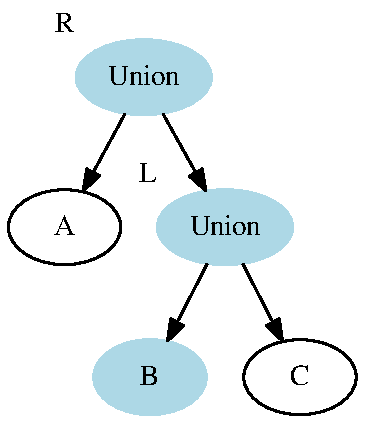
\includegraphics[scale=0.6]{figures-gen/example3.pdf} \\
L & \multicolumn{2}{c}{R} & RL \\
\multicolumn{2}{c}{last\_left\_to\_right} & \multicolumn{2}{c}{extend\_list} \\
\hline
\multicolumn{4}{c}{next\_state} \\
\end{tabular}
\caption{State-stepping operation for choice lists}
\label{fig:sstep}
\end{figure}

The first step for the iteration function is \verb|last_left_to_right|. This
function finds the final Left instance in a list of choices and converts it to
a Right instance appended to the rest of the list unmodified. The new path
therefore points to the deepest as-yet unexplored path. However, its length
may be insufficient to  make a choice at each reachable union.
\verb|extend_list| then finds where the new choice list runs out and fills it
out to be valid with respect to the type giving a valid state. If no successor
state is found---if there are no Left choices that remain---then the function
will return None.

An example of a single step on the type $\union{A}{\union{B}{C}}$ is shown in
figure~\ref{fig:sstep}. Starting from the initial choice---simply picking the
left node---\verb|last_left_to_right| turns the left choice into a right choice.
This path is invalid for this type, however, so \verb|extend_list| is needed to
initialize the remainder of the path to make it valid. To do so, it picks the 
left choice at the terminal union, producing a valid path.

\begin{verbatim}
type st_res =
  | Subtype of st_choice list * st_choice list
  | NotSubtype

let rec base_subtype (a:typ) (b:typ) (fa:st_choice list) (ex : st_choice list)
  match (a,b,fa,ex) with
  | (Atom i, Atom j, _, _) -> if i == j then Subtype(fa, ex) else NotSubtype
  | (Tuple1 t1, Tuple1 t2, _, _) -> base_subtype t1 t2 fa ex
  | (Tuple2(ta1, ta2), Tuple2(tb1, tb2), _, _) ->
     (match base_subtype ta1 tb1 fa ex with
      | Subtype(cfa, cex) -> base_subtype ta2 tb2 cfa cex
      | NotSubtype -> NotSubtype)
  | (Union(a1,a2),b,choice::fa,ex) -> 
  		base_subtype (match choice with Left -> a1 | Right -> a2) b fa ex
  | (a,Union(b1,b2),fa,choice::ex) -> 
  		base_subtype a (match choice with Left -> b1 | Right -> b2) fa ex
\end{verbatim}

\verb|base_subtype| is responsible for using two paths---one for the left and
right hand sides of the subtyping relation---and checking that the subtype
relation holds with respect to those paths. Given a basic type---an atom or a
tuple---it will either check equality or recur respectively. Given a union, it
will grab the choice to make at that union off of the choice stacks and continue
recursively. The function then returns an instance of \verb|st_res|, which
gives the remaining choice stacks if successful or nothing otherwise.

\begin{verbatim}
let rec ex_subtype (a:typ) (b:typ) (fa:st_choice list) (cex : st_choice list) =
  match base_subtype a b fa cex with
  | Subtype(_,_) -> true
  | NotSubtype-> 
     (match next_state b cex with
      | Some ns -> ex_subtype a b fa ns
      | None -> false)

let rec fa_ex_subtype (a:typ) (b:typ) (cfa:st_choice list) =
  match ex_subtype a b cfa (initial_choice b) with
  | true -> (match next_state a cfa with
               | Some ns -> fa_ex_subtype a b ns
               | None -> true)
  | false -> false

let rec subtype (a:typ) (b:typ) = fa_ex_subtype a b (initial_choice a)
\end{verbatim}

Subtyping types with distributive unions then reduces to iterating through
every combination of the two iterators for a given relation. \verb|subtype|
calls \verb|fa_ex_subtype|, which iterates through the left-hand-side's
iterator while ensuring that \verb|ex_subtype| (or exists-subtype) holds at
each step. \verb|ex_subtype| then finds if there is an instantiation of the
right-hand-side iterator where \verb|base_subtype| holds.

\begin{figure}
\center
\begin{tabular}{cc|cc|c}
\multicolumn{2}{c}{Stack} & \multicolumn{2}{c}{Type} & Base Query \\
\hline
$\forall$ & $\exists$ & $\forall$ & $\exists$ & \\
\hline
\goodcell L & \goodcell L & \goodcell 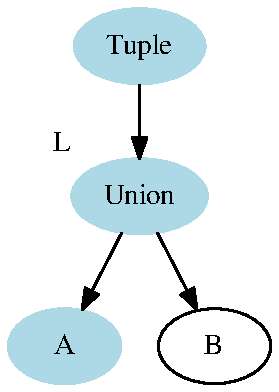
\includegraphics[scale=0.3]{figures-gen/left1.pdf} & \goodcell 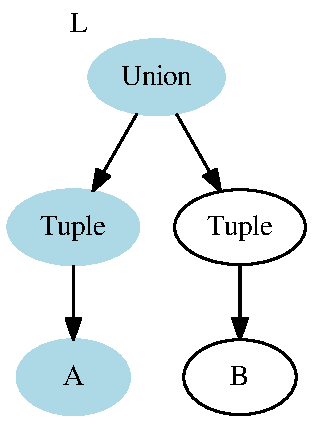
\includegraphics[scale=0.3]{figures-gen/right1.pdf} 
		& \goodcell $\tupleo{A} <: \tupleo{A}$ \\
\goodcell L & \badcell R & \badcell 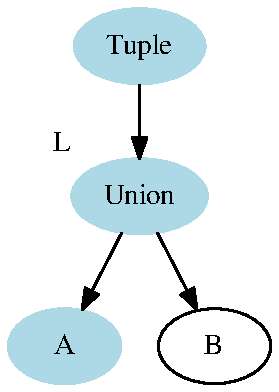
\includegraphics[scale=0.3]{figures-gen/left1.pdf} & \badcell 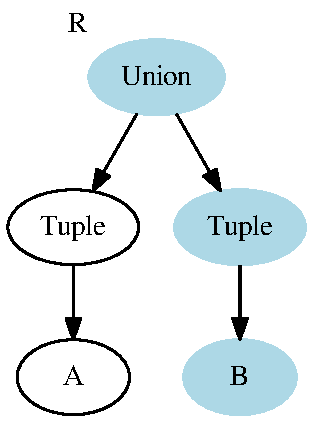
\includegraphics[scale=0.3]{figures-gen/right2.pdf}  
		& \badcell $\tupleo{A} \not<: \tupleo{B}$ \\
\hline
\goodcell R & \badcell L & \badcell 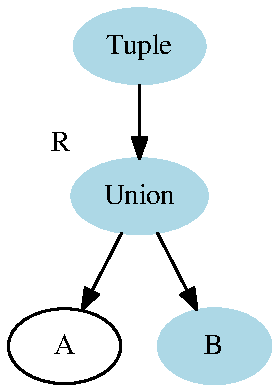
\includegraphics[scale=0.3]{figures-gen/left2.pdf} & \badcell 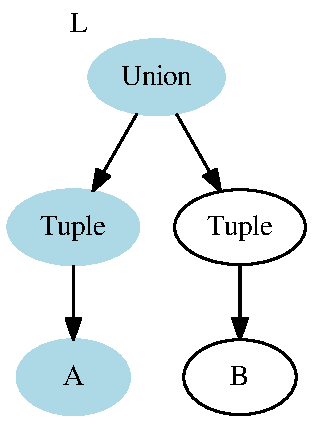
\includegraphics[scale=0.3]{figures-gen/right1.pdf}  
		& \badcell $\tupleo{B} \not<: \tupleo{A}$ \\
\goodcell R & \goodcell R & \goodcell 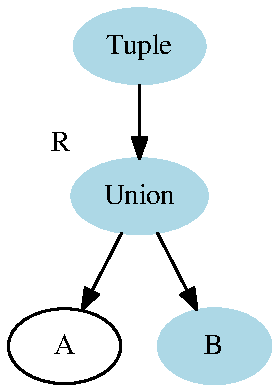
\includegraphics[scale=0.3]{figures-gen/left2.pdf} & \goodcell 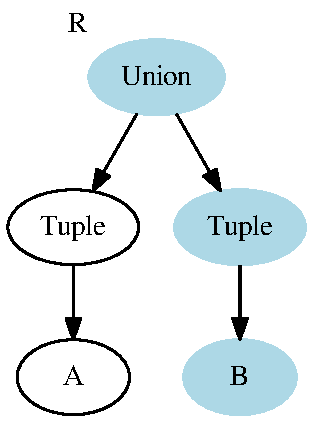
\includegraphics[scale=0.3]{figures-gen/right2.pdf}  
		& \goodcell $\tupleo{B} <: \tupleo{B}$ \\
\hline
\end{tabular}

\hspace{1em}

$\tupleo{\union{A}{B}} <: \union{\tupleo{A}}{\tupleo{B}}$

\caption{Checking for Subtype}
\label{fig:cfs}
\end{figure}

Figure~\ref{fig:cfs} shows the execution of this function when checking the
relation $\tupleo{\union{A}{B}} <: \union{\tupleo{A}}{\tupleo{B}}$. For each
instantiation of the $\forall$ choice stack, there needs to be an
instantiation  of the $\exists$ stack such that when the type is subsetted
using those stacks the subtype relation holds.

\section{Unions and Tuples}

We begin with a presentation of the algorithm on the language limited to unions
and tuples. We then describe and show the proof of correctness of the algorithm
for this language, then discuss how it can be extended to handle existential type
variables.

\begin{figure}
\begin{align*}
\xt{t} := & \xt{A},\xt{B},\xt{C},\xt{D} \\
&| \union{\xt t}{\xt t} \\
&| \tupleo{\xt t} \\
&| \tuplet{\xt t}{\xt t} \\
\end{align*}
\caption{The language of unions and tuples}
\label{fig:unionlang}
\end{figure}

In order to describe semantic subtyping for this language, we will need a
notion of type-set equivalences. For this small language, it can be defined
straightforwardly as:

\begin{align*}
\denotes{\xt{A}} &= \{A\} \\
\denotes{\union{t_1}{t_2}} &= \denotes{t1} \cup \denotes{t2} \\
\denotes{\tupleo{t}} &= \{\tupleo{t'} | t' \in \denotes{t}\} \\
\denotes{\tuplet{t_1}{t_2}} &= \{\tuplet{t'_1}{t'_2} | t_1' \in \denotes{t_1},  t_2' \in \denotes{t_2'}\} \\
\end{align*}

We want to be able to decide semantic subtyping relations for this language,
defined as if $\denotes{t_1} \subseteq \denotes{t_2}$, then $t_1 <: t_2$. This
leads us to definition~\ref{dfn:scr} as our correctness criteria for subtyping
relations.

\begin{definition}[Subtyping Correctness]
A subtyping relation $<:$ is correct if $t_1 <: t_2$ iff $\forall t_1' \in \denotes{t_1},
\exists t_2' \in \denotes{t_2}, t_1 \bsub t_2$.
\label{dfn:scr}
\end{definition}

This definition of subtyping is canonicalized in our Coq proof as the
\texttt{NormalSubtype} relation. A correct subtyping algorithm \texttt{subtype} in Coq
will have the type \verb|forall t1 t2:type, {NormalSubtype t1 t2} + {~NormalSubtype t1 t2}|,
indicating that for any pair of types, it can decide whether they are or are not a subtype 
under definition~\ref{dfn:scr}.

The classical subtyping relation for unions does not satisfy
definition~\ref{dfn:scr}, even on this limited type language. We depict the
standard definition of subtyping in figure~\ref{fig:typsub}. The problem with
this definition arises from the combination of unions and tuples in non-normal
form.

\begin{figure}
\begin{mathpar}
\inferrule{ }{A \bsub A}

\inferrule{t \bsub t_1}{t \bsub \union{t_1}{t_2}}

\inferrule{t \bsub t_2}{t \bsub \union{t_1}{t_2}}

\inferrule{t_1 \bsub t \\ t_2 \bsub t}{\union{t_1}{t_2} \bsub t}

\inferrule{t_1 \bsub t_2}{\tupleo{t_1} \bsub \tupleo{t_2}}

\inferrule{t_1 \bsub t_2 \\ t_1' \bsub t_2'}{\tuplet{t_1}{t_1'} \bsub \tuplet{t_2}{t_2'}}
\end{mathpar}
\caption{Typical subtyping rules for tuples and unions}
\label{fig:typsub}
\end{figure}

To illustrate the problem, consider deciding the subtyping relation
$\tupleo{\union{\xt{A}}{\xt{B}}} <: \union{\tupleo{\xt{A}}}{\tupleo{\xt{B}}}$.
If we look at it denotationally, it is evident that
$\denotes{\tupleo{\union{\xt{A}}{\xt{B}}}} =
\{\tupleo{\xt{A}},\tupleo{\xt{B}}\}$, that
$\denotes{\union{\tupleo{\xt{A}}}{\tupleo{\xt{B}}}} =
\{\tupleo{\xt{A}},\tupleo{\xt{B}}\}$, and therefore that the subtyping
relation should hold. However, if we attempt to use the above rules to decide
this subtyping relation, we end up with one of two faulty derivations:

\begin{mathpar}
\inferrule*{
		\inferrule*{
				\inferrule*{\xt{A} \bsub \xt{A} \\ \xt{B} \not\bsub \xt{A}}{\union{\xt{A}}{\xt{B}} \bsub \xt{A}}} 
		{\tupleo{\union{\xt{A}}{\xt{B}}} \bsub \tupleo{\xt{A}}}}
{\tupleo{\union{\xt{A}}{\xt{B}}} \bsub \union{\tupleo{\xt{A}}}{\tupleo{\xt{B}}}}

\inferrule*{
		\inferrule*{
				\inferrule*{\xt{A} \not\bsub \xt{B} \\ \xt{B} {\bsub} \xt{B}}{\union{\xt{A}}{\xt{B}} \bsub \xt{B}}} 
		{\tupleo{\union{\xt{A}}{\xt{B}}} \bsub \tupleo{\xt{B}}}}
{\tupleo{\union{\xt{A}}{\xt{B}}} \bsub \union{\tupleo{\xt{A}}}{\tupleo{\xt{B}}}}
\end{mathpar}

The problem with this relation is that the straightforward algorithm ``jumps
to conclusions'' about what choice is to be made for the union on the right
hand side. Eventually, it reaches a point where whatever choice is made at the
top level is invalidated.

To solve this problem, other approaches normalize the type on the left hand
side, bringing the union to the outermost position. Normalization will convert
the relation to $\union{\tupleo{\xt{A}}}{\tupleo{\xt{B}}} \bsub
\union{\tupleo{\xt{A}}}{\tupleo{\xt{B}}}$, and the relation will hold. However,
all unions within the type must be eliminated in this process, and therefore all 
possible choices of the unions must be expanded. As a result, the size of the 
types under consideration becomes exponential in the number of unions within
the types and the algorithm needs exponential space to store the types being
compared.

We present an algorithm to decide subtyping relations for this type language
that is able to satisfy the correctness criteria and is able to successfully
determine that these two types are subtypes. Moreover, this algorithm is able
to decide subtyping for this language using linear space (though exponential
time) over the number of unions in the type.

\subsection{Normalization}

In order to correctly decide subtyping, it is necessary to explore each decision
made at each union. First, we will examine how normalization accomplishes this,
then describe how our iterator-or-stack based approach achieves the same result
without needing to store or generate a large type.

To enable the typical algorithm to explore all possible choices at unions, the
normalization approach lifts all unions to the top level. To do this, it
computes the set of types corresponding to all possible choices for unions
embedded in the term, then adds a top-level union that enables the selection
of any one of the choices. 

For this simple type language, normalization is equivalent to computing the
denotation set for the type. We define a metafunction \texttt{normalize}:

\[
\xt{normalize}(t) = \xt{Union}\{\denotes{t}\}
\]

For convenience of notation, we elide the nested unions that would be needed
if $|\denotes{t}| > 2$ and that if $|\denotes{t}| = 1$ then no union will be
generated.

We can then define a correct semantic subtyping relation for our type
language using this metafunction. (TODO: subscript the subtype relations)

\begin{mathpar}
\inferrule{\xt{normalize}(t_1) \bsub \xt{normalize}(t_2)}{t_1 \nsub t_2}
\end{mathpar}

This normalization-based subtyping relation satisfies definition~\ref{dfn:scr}.

\begin{theorem}[Correctness of Normalization-Based Subtyping]
$t_1 \nsub t_2$ iff $\forall t_1' \in \denotes{t_1},
\exists t_2' \in \denotes{t_2}, t_1 \bsub t_2$
\end{theorem}
\begin{proof}
See the Coq implementation of \verb|normalize_subtype|. 
\end{proof}

However, the normalization process is both space intensive (as all unions must
be expanded) and is incompatible with the existential type variables that will
be introduced later. To address these issues, we present an algorithm that can
decide correct subtyping without needing to expand the types being compared.

\subsection{Iterators}

To explain the operation of the iterator-based algorithm for subtyping, we
will begin with an examination of how the normalization algorithm actually
decides subtyping. Consider the original problematic relation 
$\tupleo{\union{\xt{A}}{\xt{B}}} \nsub \union{\tupleo{\xt{A}}}{\tupleo{\xt{B}}}$, which
is expanded by normalization to $\union{\tupleo{\xt{A}}}{\tupleo{\xt{B}}} \bsub
\union{\tupleo{\xt{A}}}{\tupleo{\xt{B}}}$. The normalization process brought all inner
unions to the top level, which allowed the basic subtyping algorithm to examine all options
without running into structural limitations.

The iterator-based algorithm for subtyping replaces normalization (computing all options
in one go) with an incremental approach to exploring choices made at unions. It represents
a specific set of choices at a union as a state of an iterator, which will iterate through
all possible choices of union. On top of this, we can define an algorithm for deciding correct
subtyping.

\subsubsection{Infrastructure}

We have implemented the iterator-based subtyping algorithm in Coq, and will
present its implementation.

\begin{verbatim}
Inductive TypeIterator: type -> Set :=
| TIAtom : forall i, TypeIterator (atom i)
| TITuple1 : forall tp, TypeIterator tp -> TypeIterator (tuple1 tp)
| TITuple2 : forall t1 t2, TypeIterator t1 -> TypeIterator t2 -> TypeIterator (tuple2 t1 t2)
| TIUnionL : forall t1 t2, TypeIterator t1 -> TypeIterator (union t1 t2)
| TIUnionR : forall t1 t2, TypeIterator t2 -> TypeIterator (union t1 t2).
\end{verbatim}

Members of the \verb|TypeIterator t| type are iterator states for a type
\verb|t|. An iterator state is a traversal of the type tree from the root to a leaf
(for our type language, an atom), and each state describes a set of choices to take
at each union (denoted by \verb|TIUnionL| and \verb|TIUnionR|). Using a \verb|TypeIterator t|,
we can subset a source type to eliminate all unions (which we denote as the current type) with
a function as follows:

\begin{verbatim}
Fixpoint current (t:type)(ti:TypeIterator t):type :=
match ti with
| TIAtom i => atom i
| TITuple1 tip p => tuple1 (current tip p)
| TITuple2 ti1 ti2 p1 p2 => tuple2 (current ti1 p1) (current ti2 p2)
| TIUnionL ti1 ti2 pl => (current ti1 pl)
| TIUnionR ti1 ti2 pr => (current ti2 pr)
end.
\end{verbatim}

Next, we need to define the operations that make a \verb|TypeIterator| into an actual
iterator. In particular, we need to be able to find an initial state and then a function
that steps through all possible states from that initial state. We define our initial state
as the state where we only take the leftmost branch on all unions, and then steps ``rightize''
the iterator from there.

\begin{verbatim}
Fixpoint start_iterator (t:type):TypeIterator t :=
  match t with
  | (atom i) => TIAtom i
  | (tuple1 t) => TITuple1 t (start_iterator t)
  | (tuple2 t1 t2) => TITuple2 t1 t2 (start_iterator t1) (start_iterator t2)
  | (union t1 t2) => TIUnionL t1 t2 (start_iterator t1)
  end.
\end{verbatim}

Correctness for \verb|start_iterator| is simple.

\begin{theorem}
Every type in $\denotes{t}$ will be explored by \verb|start_iterator t| 
\end{theorem}
\begin{proof}
See \verb|iterator_has_clauses| in the Coq proof.
\end{proof}

\begin{verbatim}
Fixpoint next_state (t:type)(ti:TypeIterator t) : option (TypeIterator t) :=
  match ti with
  | TIAtom i => None
  | TITuple1 tip p => option_map (TITuple1 tip) (next_state tip p)
  | TITuple2 ti1 ti2 p1 p2 =>
    match (next_state ti2 p2) with
    | Some np2 => Some(TITuple2 ti1 ti2 p1 np2)
    | None =>
      match (next_state ti1 p1) with
      | Some np1 => Some(TITuple2 ti1 ti2 np1 (start_iterator ti2))
      | None => None
      end
    end
  | TIUnionL ti1 ti2 pl =>
    match (next_state ti1 pl) with
    | Some npl => Some(TIUnionL ti1 ti2 npl)
    | None => Some(TIUnionR ti1 ti2 (start_iterator ti2))
    end
  | TIUnionR ti1 ti2 pr => option_map (TIUnionR ti1 ti2) (next_state ti2 pr)
  end.
\end{verbatim}

\verb|next_state| returns \verb|Some s| if there is some successor state
\verb|s| to the current, and \verb|None| if the given iterator state is
terminal. It will go left-to-right through unions, and will explore 2-tuples
by iterating through the choices on the right for each choice on the left.
This definition leads us to the Coq induction principle over iterators.

\begin{theorem}
\begin{verbatim}
Definition iter_rect
  (t:type) (P:TypeIterator t -> Set)
           (pi: forall it, next_state t it = None -> P it)
           (ps : forall it' it'', P it'' -> next_state t it' = Some it'' -> P it')
           (it : TypeIterator t) : P it  
\end{verbatim}

For any type \verb|t| and proposition \verb|P|, and if:
\begin{itemize} 
	\item \verb|P| holds for an iterator that has no next state (e.g. is done)
	\item if \verb|P| holds for the \emph{following} iterator state \verb|it|,
	then \verb|P| holds for the \emph{preceeding} iterator state \verb|it'|.
\end{itemize}
Then \verb|P| holds for all iterators for type \verb|t|
\end{theorem}
\begin{proof}
See the Coq proof for this paper.
\end{proof}

This definition provides us with both a useful correctness property as well as
a termination argument, as the principle is in \verb|Set|. We use this
induction principle to define decidable implementations of subtyping using
iterators. For details  of this use, see the associated Coq code.

The correctness properties we are interested in require reasoning about the
entire set of types that is explored by the iterator. As a result, we need a
propoisitional form that describes all types that remain to be explored by the
iterator, which we refer to as  \verb|Remaining|. We will not provide the
complete definition of \verb|Remaining| here,  but the informal definition is
that if \verb|Remaining t it l|, then the type iterator \verb|it| for type
\verb|t| will encounter \verb|l| different types before it can no longer be
stepped.  

\subsubsection{Subtyping with Iterators}

With this, we can define the core decision procedures of the subtyping
algorithm. We will first define the right-hand-side check, the exists check,
that for some fixed left-hand-side type finds if there exists some instantiation
on the right hand side that is a subtype. Then, we will use this to define the overall
subtyping algorithm, which checks that for every instantiation on the left hand side
there exists an instantiation on the right hand side.

To show correctness of the exists check (on the right hand side) algorithm, we will
prove an inner property (that is well-suited to our induction principle), then use that
lemma to show that there is a decision procedure for the full exists-side check. The 
inner property we desire is that for any iterator state \verb|it| of type \verb|t|, it
is possible to decide whether the iterator will encounter an element that is a supertype
of the left-hand-side or not. In Coq, this is represented as

\begin{verbatim}
Definition exists_iter_inner(a b : type)(it:TypeIterator b) :
  ({ t | forall l, Remaining b it l -> In t l /\ BaseSubtype a t } +
   {forall t l, Remaining b it l -> In t l -> ~(BaseSubtype a t) }).
\end{verbatim}

Using this - and knowing that we can prove that \verb|start_iterator| has
every type choice possible remaining - we can show that we can decide whether
any possible choice of type \verb|b| is a supertype of our reference type
\verb|a| on the left-hand-side or not. This decision procedure is \verb|exists_iter|,
and for implementation details see the Coq proof.

\begin{verbatim}
Definition exists_iter(a b : type) : 
  ({ t | InType t b /\ BaseSubtype a t } +
   {forall t, InType t b -> ~(BaseSubtype a t) }).
\end{verbatim}

We can then prove equivalent decision procedures for the left-hand-side of the
relation. We now want to prove that for every choice we make on the left-hand-side,
there exists some choice that produces a supertype on the right-hand-side. 

\begin{verbatim}
Definition forall_iter_inner (a b : type) (it : TypeIterator a) :
  { forall l, Remaining a it l ->
              forall t, In t l ->
                        exists t', InType t' b /\ (BaseSubtype t t')} +
  { forall l, Remaining a it l ->
              exists t, In t l /\ forall t', InType t' b -> ~ (BaseSubtype t t')}.
\end{verbatim}

We then use this to prove the final iterator, running the intermediate result from
the initial state:

\begin{verbatim}
Definition forall_iter (a b : type) :
  { forall t, In t (clauses a) -> exists t', InType t' b /\ (BaseSubtype t t')} +
  { exists t, In t (clauses a) /\ forall t', InType t' b -> ~ (BaseSubtype t t')}.
\end{verbatim}

Finally, we can define a decidable function (called \verb|subtype| in the proof)
that decides whether two types are subtypes or not. \verb|subtype| simply invokes
\verb|forall_iter| to decide subtyping.

\begin{verbatim}
Definition subtype(a b:type) : {NormalSubtype a b} + {~NormalSubtype a b}.
  destruct (forall_iter a b).
  - left. [...]
  - right. [...]
Defined.
\end{verbatim}

Therefore, using iterators, we can decide whether subtyping holds for any two types
in our language. We will now show an equivalence between iterators and stacks-of-choices,
allowing for more efficient implementation.

\subsection{Stacks-as-Iterators}

The equivalence of stacks (or lists of choices) and type iterators arises from
the design of our iterators. Each iterator state represents a set of choices
made at each  union inside the type, choices that could also be recorded as
simple boolean values. If we fix the type under consideration and perform an
inorder traversal of the iterator, we can construct a bijective mapping
between instances of \verb|TypeIterator t| and  \verb|list bool|. We can then
use this mapping to define and prove correct an alternative algorithm for
deciding subtyping for our type language that does not need the full iterator.

To start with, we will begin by describing the mapping between iterators and
stacks (or lists of choices). In the accompanying Coq code, we define
\verb|st_context| (or subtype contexts) as \verb|list bool|.

\subsubsection{Equivalence}

To illustrate the equivalence between choice stacks and iterators, we will
first present the \verb|lookup_path| and \verb|iterator_to_path| operations;
these operations lookup the current type based on a path and which convert an
iterator to a choice stack, respectively. 

\begin{verbatim}
Fixpoint lookup_path(t:type)(p:st_context) : type * st_context :=
  match t, p with
  | atom i, _ => (t, p)
  | tuple1 t, _ => let (r,p) := lookup_path t p in (tuple1 r, p)
  | tuple2 t1 t2, _ =>
    let (r1,p1) := lookup_path t1 p in
    let (r2,p2) := lookup_path t2 p1 in
    (tuple2 r1 r2, p2)
  | union l r, false::rs => lookup_path l rs
  | union l r, true::rs => lookup_path r rs
  | _, nil => (t, nil)
  end.
\end{verbatim}

\verb|lookup_path| takes both a type and a subtype context (or choice stack)
and returns the combination of the now-unionless type and whatever of the
choice stack was left over. This ``tail'' is necessary in order to handle
tuples, whose right branch is now simply concatenated onto the left branch's
choice stack (and is therefore a postfix of the left branch's). Comparing
\verb|lookup_path| (for choice stacks) and \verb|current| (for iterators), 
they share the same structure. The only differences are the sequential handling
of tuples and the use of the choice stack instead of TIUnionL/TIUnionR for
choosing branches of unions.

\begin{verbatim}
Fixpoint iterator_to_path(t:type)(it:TypeIterator t):st_context :=
   match it with
   | TIAtom _ => nil
   | TITuple1 tp it1 => iterator_to_path tp it1
   | TITuple2 t1 t2 it1 it2 => (iterator_to_path t1 it1) ++ (iterator_to_path t2 it2)
   | TIUnionL t1 _ it1 => false :: (iterator_to_path t1 it1)
   | TIUnionR _ t2 it1 => true :: (iterator_to_path t2 it1)
   end.
\end{verbatim}

With this similarity in mind, we can now look at how to convert an iterator to
a choice stack, implemented as \verb|iterator_to_path|. The conversion
proceeds structurally, with tuples-equivalent-stacks concatenated onto one
another and union choices producing false (for left-choice) and true (for
right-choice). These definitions then let us pose a basic correctness theorem
for this new representation:

\begin{lemma}[Iterator to path is correct]
\begin{verbatim}
Lemma itp_correct : forall t it, current t it = fst (lookup_path t (iterator_to_path t it)).
\end{verbatim}

For every type \verb|t| and type iterator \verb|it|, the iterator's current type \verb|current t it| is equal
to the result of looking up the conversion of \verb|it| to a choice stack.
\end{lemma}
\begin{proof}
See \verb|itp_correct| in the Coq proof.
\end{proof}

\subsubsection{Stepping}

We now need an equivalent of \verb|next_state| for choice stacks. Choice stacks
are hard to iterate, as their length can change as they are stepped and therefore
simple binary-number style stepping is insufficient. Instead, we implement stepping
for choice stacks with two functions which compose into the desired step function.

\begin{verbatim}
Fixpoint flip_last_left(ls:st_context):=
  match ls with
  | false::rs =>
    match flip_last_left rs with
    | Some s => Some(false :: s)
    | None => Some(true::nil)
    end
  | true::rs =>
    match flip_last_left rs with
    | Some s => Some(true::s)
    | None => None
    end
  | nil => None
  end.

Fixpoint extend_list(t:type)(ls:st_context) :=
  match t,ls with
  | atom i, _ => (nil, ls)
  | tuple1 t, _ => extend_list t ls
  | tuple2 t1 t2, _ =>
    let (hd1,tl1) := extend_list t1 ls in
    let (hd2,tl2) := extend_list t2 tl1 in
    (hd1 ++ hd2, tl2)
  | union l r, false::rs => extend_list l rs
  | union l r, true::rs => extend_list r rs
  | union l r, nil =>
    let (hd,tl) := extend_list l nil in (false :: hd, tl)
  end.

Definition step_ctx (t : type) (pth:st_context) : option st_context := 
	option_map (fun x => x ++ (fst (extend_list t x))) (flip_last_left pth).
\end{verbatim}

\verb|flip_last_left| flips the final left (or false) in a subtype
context into a right choice in that union, then truncates the choice 
stack to that flipped position. This operation causes the implied iterator
to move to the deepest possible alternative type.

\verb|extend_list| pads out a given subtype context with left-choices to be a
valid context for the given path. It will fill out a subtype environment that
has made an alternate choice at a branch node and therefore needs to traverse
the rest of the type tree. We combine these two operations to define
\verb|step_ctx|, which flips the final left choice in the given context then
extends the context to be valid for the iterated type.

Correctness for \verb|step_ctx| is expressed in terms of the iterator
\verb|next_step| operation and the \verb|iterator_to_path| operation.

\begin{lemma}[Correctness of step\_ctx]
\begin{verbatim}
forall t it,
    step_ctx t (iterator_to_path t it) =
    (option_map (iterator_to_path t) (next_state t it)).
\end{verbatim}
For every type \verb|t| and type iterator \verb|it|,
stepping the choice-list equivalent of \verb|it| will
produce the same result as converting the result of stepping
\verb|it|.
\end{lemma}
\begin{proof}
See \verb|list_step_correct| in the Coq proof.
\end{proof}

We can then define the exists and forall-exists subtype decision procedures
on top of the \verb|step_ctx| and \verb|lookup_path| operations:

\begin{verbatim}
Fixpoint ex_subtype (a b : type)(cex :st_context)(fuel:nat) : option bool :=
  match base_subtype a (fst (lookup_path b cex)) with
  | left _ => Some true
  | right _ =>
    match step_ctx b cex with
    | Some ns =>
      match fuel with
      | S n => ex_subtype a b ns n
      | 0 => None
      end
    | None => Some false
    end
  end.

Fixpoint fa_ex_subtype (a b : type)(cfa : st_context)(fuel:nat) : option bool :=
  match fuel with
  | S n =>
    match ex_sub_ex (fst (lookup_path a cfa)) b with
    | true =>
      match step_ctx a cfa with
      | Some ns => fa_ex_subtype a b ns n
      | None => Some true
      end
    | _ => Some false
    end
  | 0 => None
  end.
\end{verbatim}

The functions \verb|ex_subtype| and \verb|fa_ex_subtype| are direct choice stack equivalents
of the iterator-based \verb|exists_iter| and \verb|forall_exists_iter|. This then leads to
a correctness theorem for the choice stack versions.

\begin{lemma}[Correctness of existential subtype checking with choice stacks]
\begin{verbatim}
forall a b it, 
  (exists pf, exists_iter_inner a b it = inleft pf) <->
   exists n, ex_subtype a b (iterator_to_path b it) n = Some true.
\end{verbatim}
For every two types \verb|a| and \verb|b|, the iterator-based algorithm
\verb|exists_iter_inner| will produce a proof that \verb|a| is a subtype
of \verb|b| if and only if there is an integer \verb|n| such that
 \verb|ex_subtype| given \verb|n| fuel runs producing true.
\end{lemma}
\begin{proof}
See \verb|ex_sub_corr_eq| in the Coq proof.
\end{proof}

\begin{lemma}[Correctness of forall-exists subtype checking with choice stacks]
\begin{verbatim}
forall a b it,
   (exists pf, forall_iter_inner a b it = left pf) <->
    exists n, fa_ex_subtype a b (iterator_to_path a it) n = Some true.
\end{verbatim}
For every two types \verb|a| and \verb|b|, the iterator-based algorithm
\verb|forall_iter_inner| will produce a proof that \verb|a| is a subtype
of \verb|b| if and only if there is an integer \verb|n| such that
 \verb|fa_ex_subtype| given \verb|n| fuel runs producing true.
\end{lemma}
\begin{proof}
See \verb|fa_sub_corr_eq| in the Coq proof.
\end{proof}

The choice stack-based algorithm produces the same results as the 
iterator-based algorithm. 

\bibliographystyle{plain}
\bibliography{refs}

\end{document}
